\begin{figure}[htbp]
\centering
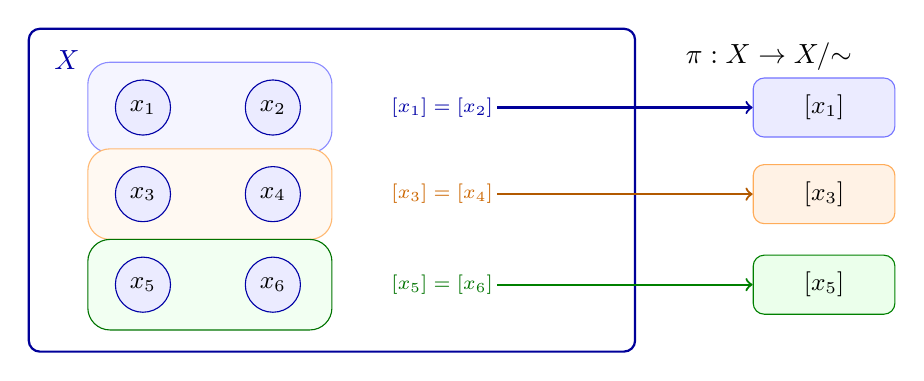
\begin{tikzpicture}[font=\small,element/.style={circle,draw=blue!65!black,fill=blue!8,minimum size=0.7cm},class/.style={draw=gray!60,fill=gray!5,rounded corners,minimum width=1.8cm,minimum height=0.75cm}]
    \draw[rounded corners,thick,draw=blue!60!black] (0,0) rectangle (7.7,4.1);
    \node[anchor=north west,font=\bfseries,text=blue!65!black] at (0.2,3.95) {$X$};
    \node[draw=blue!45,fill=blue!4,rounded corners=8pt,minimum width=3.1cm,minimum height=1.15cm] at (2.3,3.1) {};
    \node[draw=orange!55,fill=orange!5,rounded corners=8pt,minimum width=3.1cm,minimum height=1.15cm] at (2.3,2.0) {};
    \node[draw=green!45!black,fill=green!5,rounded corners=8pt,minimum width=3.1cm,minimum height=1.15cm] at (2.3,0.85) {};
    \node[element] at (1.45,3.1) {$x_1$};\node[element] at (3.1,3.1) {$x_2$};
    \node[element] at (1.45,2.0) {$x_3$};\node[element] at (3.1,2.0) {$x_4$};
    \node[element] at (1.45,0.85) {$x_5$};\node[element] at (3.1,0.85) {$x_6$};
    \node[font=\scriptsize,text=blue!65!black] at (5.25,3.1) {$[x_1]=[x_2]$};
    \node[font=\scriptsize,text=orange!80!black] at (5.25,2.0) {$[x_3]=[x_4]$};
    \node[font=\scriptsize,text=green!45!black] at (5.25,0.85) {$[x_5]=[x_6]$};
    \node[font=\bfseries] at (9.4,3.75) {$\pi:X\to X/{\sim}$};
    \node[class,draw=blue!55,fill=blue!8] (q1) at (10.1,3.1) {$[x_1]$};
    \node[class,draw=orange!65,fill=orange!10] (q2) at (10.1,2.0) {$[x_3]$};
    \node[class,draw=green!50!black,fill=green!8] (q3) at (10.1,0.85) {$[x_5]$};
    \draw[->,thick,blue!60!black] (5.95,3.1) -- (q1.west);
    \draw[->,thick,orange!70!black] (5.95,2.0) -- (q2.west);
    \draw[->,thick,green!50!black] (5.95,0.85) -- (q3.west);
\end{tikzpicture}
\caption{An equivalence relation partitions $X$ into disjoint classes. The quotient set has one element for each class, and the quotient map sends every member of a block to that class.}
\label{fig:equivalence-partition-quotient}
\end{figure}